\documentclass[a4paper,12pt]{article}

\usepackage{cmap}					
\usepackage[T2A]{fontenc}
\usepackage[utf8]{inputenc}
\usepackage[english,russian]{babel}
\usepackage{hyperref}
\usepackage{graphicx}

\hypersetup{
    colorlinks=true,
    linkcolor=blue,
    filecolor=magenta,      
    urlcolor=cyan,
}

\usepackage{amsmath,amsfonts,amssymb,mathtools}
\usepackage{icomma}

\usepackage{euscript}
\usepackage{mathrsfs}
\usepackage{graphicx}
\usepackage{eso-pic}

\graphicspath{ {images/} }

\title{Одномерные Методы Оптимизации. Лабораторная работа №1}
\author{Раков Николай, Булкина Милена}
\date{}

\begin{document}

\maketitle
\clearpage

\section{Постановка задания}

Реализовать и протестировать следующие алгоритмы одномерной минимизации функции:

\begin{itemize}
\item Метод Дихотомии
\item Метод Золотого Сечения
\item Метод Фибоначчи
\item Метод Парабол
\item Комбинированный Метод Брента
\end{itemize}

\section{Исследование функции}

Вариант 8. Исходная функция
\begin{equation*}
    f(x)=-3x\sin(0.75x)+e^{-2x}
\end{equation*}

Найдём производную и приравняем нулю

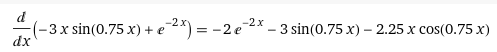
\includegraphics[width=100mm]{wa3.PNG}

Найденный минимум при помощи WolframAlpha

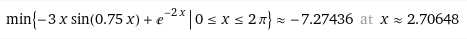
\includegraphics[width=100mm]{wa1.PNG}

Рассмотрим график функции

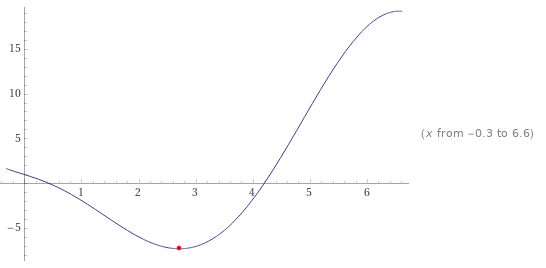
\includegraphics[width=100mm]{wa2.PNG}

\section{Результаты исследований}
При $\varepsilon=0.001$

\subsection{Метод Дихотомии}
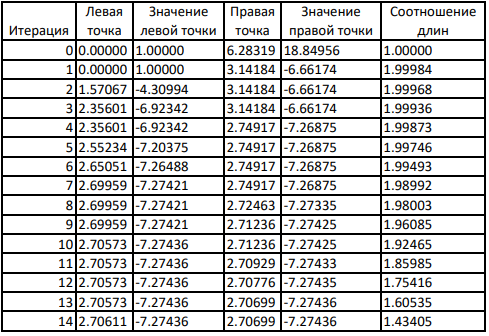
\includegraphics[width=\linewidth]{table_dichotomy.PNG}
\clearpage

\subsection{Метод Золотого Сечения}
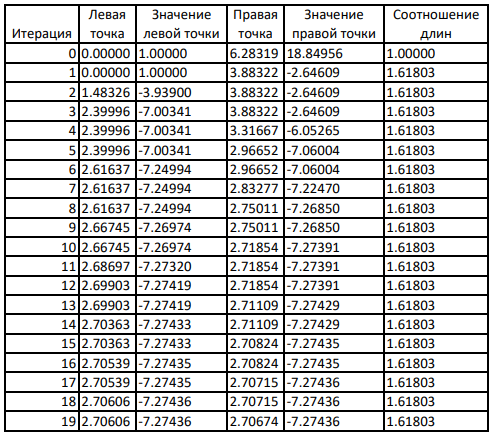
\includegraphics[width=\linewidth]{table_golden_ratio.PNG}
\clearpage

\subsection{Метод Фибоначчи}
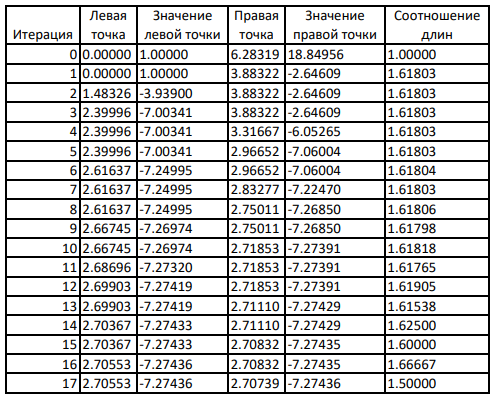
\includegraphics[width=\linewidth]{table_fibonacci.PNG}
\clearpage

\subsection{Метод Парабол}
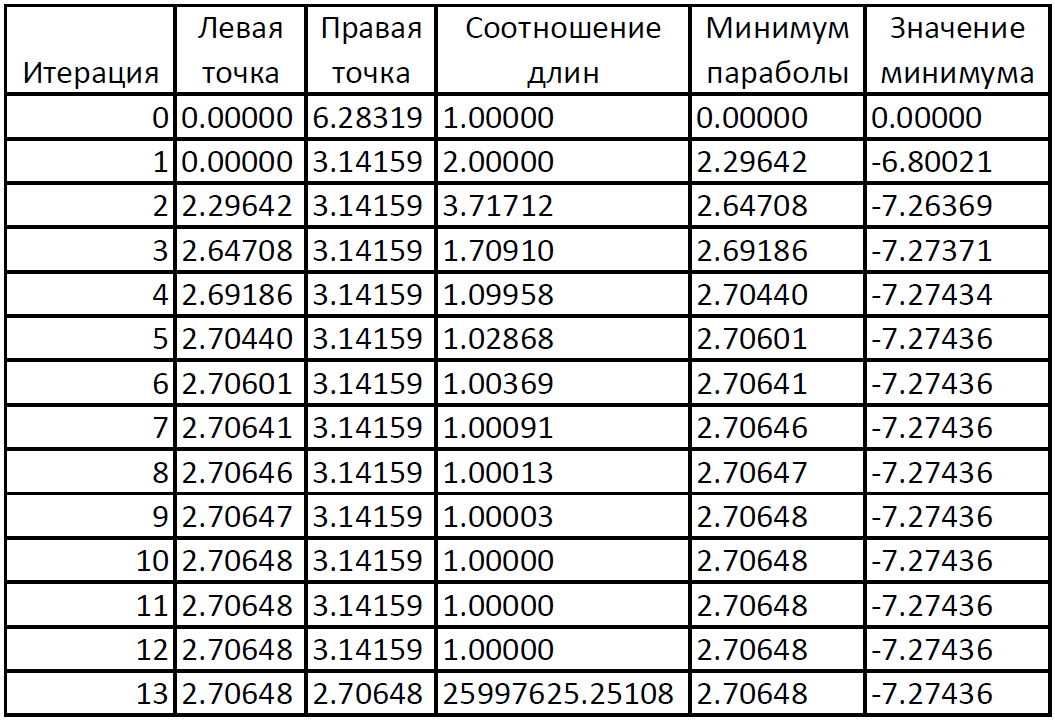
\includegraphics[width=\linewidth]{table_parabola.PNG}
\clearpage

\subsection{Комбинированный Метод Брента}
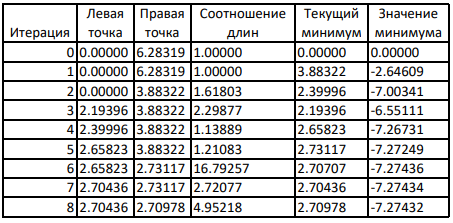
\includegraphics[width=\linewidth]{table_brent.PNG}
\clearpage

\section{Сравнение методов}
Сравним методы по количеству вычислений минимизируемой функции
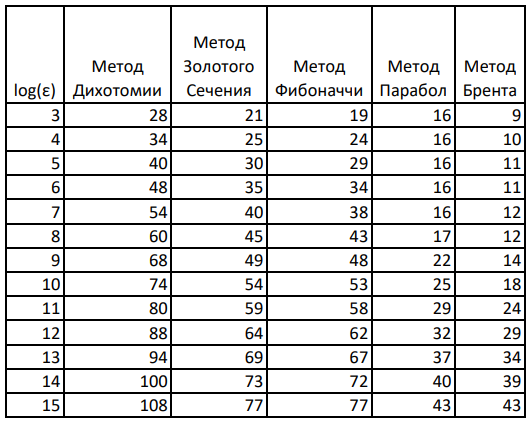
\includegraphics[width=\linewidth]{table_comp1.PNG}
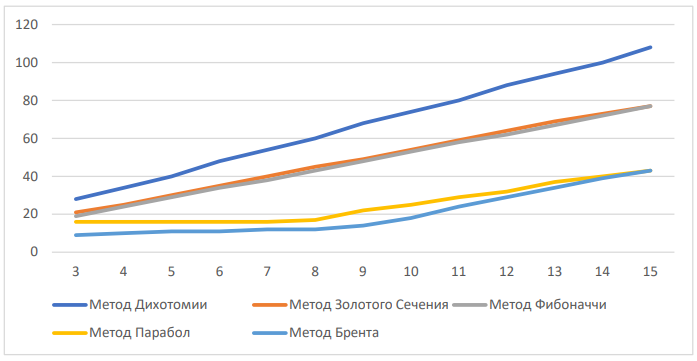
\includegraphics[width=\linewidth]{table_comp2.PNG}

Из проведённых экспериментов следует, что на исследумой функции наиболее эффективными методами минимизации являются метод Брента и метод парабол.

Рассмотрим более подробно каждый метод
\begin{itemize}
\item Метод Дихотомии - самый простой в реализации, на каждой итерации интервал неопределённости сокращается примерно в 2 раза, однако вычисляет исследуемую функцию по 2 раза за итерацию, что может оказаться критично
\item Метод Золотого Сечения - является улучшением метода дихотомии, теперь отрезок делится в пропорции золотого сечения, поэтому на каждой итерации достаточно пересчитывать одно значение функции
\item Метод Фибоначчи - является улучшением метода золотого сечения, теперь отрезок сокращается в непостоянное количество раз
\item Метод Парабол - аппроксимирует исходную функцию при помощи квадратичной. Высокая скорость сходимости гарантируется только в малой окрестности точки минимума.
\item Комбинированный Метод Брента - является комбинацией метода парабол и метода парабол.
\end{itemize}

\clearpage

\section{Тестирование алгоритмов для задач минимизации многомодальных функций}
\subsection{$x\sin(x)$ на $[-10, 10]$}
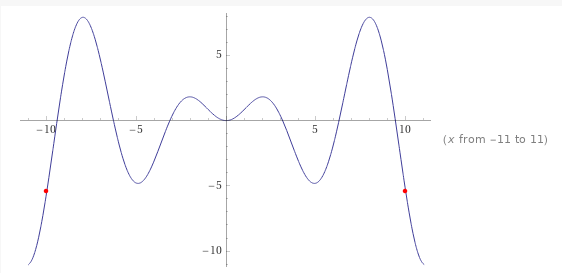
\includegraphics[width=\linewidth]{xsinx1.PNG}
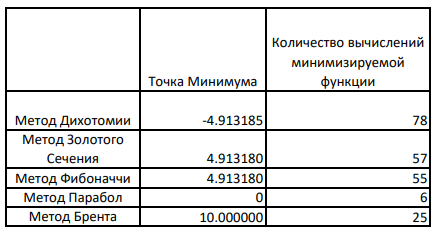
\includegraphics[width=\linewidth]{xsinx2.PNG}

\subsection{$6x^4 - 15x^3 - 2x^2 + 13x+ 10$ на $[-2, 2]$}
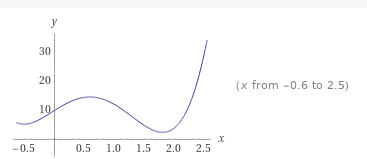
\includegraphics[width=\linewidth]{poly1.PNG}
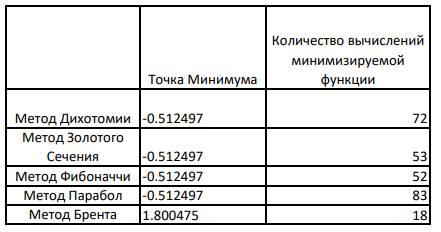
\includegraphics[width=\linewidth]{poly2.PNG}

\subsection{Вывод}
Каждый из алгоритмов находит какой-то локальный минимум, работая как с унимодальной функцией, а потому их нельзя использовать для поиска глобального минимума многомодальной функции.

\section{Выводы}
В ходе лабораторной работы были исследованы пять методов одномерной оптимизации. На унимодальным функциях лучше всего себя проявили метод Брента и метод парабол, метод дихотомии потребовал больше всего вычислений исходной функции. Эти методы оказались непременимы для минимизации многомодальных функций.
\end{document}
